\section{Motivation}

We saw in Section \ref{sec:imit} that imitation learning is broadly solved in two different ways. One approach is to pose it as a supervised learning problem where a classifier learns the action labels for all states in the state space based on training data - the expert's demonstrations. The other approach is a model-based solution that uses inverse reinforcement learning (IRL) to find a mapping from states to real-valued rewards that makes the expert trajectories seem optimal. The learner hence follows the optimal policy on these rewards. IRL methods have the advantage of representing the acquired knowledge succinctly as rewards over the states.

In practice, both these approaches could suffer from a considerable \textbf{burden on the teacher} who is expected to produce sufficient trajectories for accurate imitation. What makes this more undesirable is that many of the trajectories happen to be redundant and yet expensive. To address this, it wouldbe of interest to study active learning approaches to imitation learning. In active learning, the learner actively chooses points from a pool of unlabelled data, and requests the expert for the label. 

In model-free imitation learning techniques, the states from the pool of points and the expert action at that states would be the label. \citet{DBLP:conf/uai/JudahFD12} (Section \ref{sec:judah_active}) have proposed active learning algorithms for supervised learning based imitation learning and analyse the performance of these algorithms with respect to the performance guarantees provided by the active learning algorithm used for the classification. 


On the other hand, there has been very little work on \textit{formally} understanding active imitation learning through IRL. \citet{DBLP:conf/icra/SilverBS12} (Section \ref{sec:navigation}) have studied active learning heuristics where the learner requests trajectories in such a way that the knowledge about the reward function acquired is either novel or reduces uncertainty in the current beliefs.   \citet{DBLP:conf/pkdd/MeloL10} (Section \ref{sec:active_bayesian}) use the power of Bayesian IRL (\citet{Ramachandran:2007:BIR:1625275.1625692}, Section \ref{sec:bayesian}) to provide an empirical technique to actively query by choosing states. The state that is chosen to be queried is one which has the greatest entropy in the posterior distribution over the policy which is in turn derived from a posterior distribution over the rewards as computed by the Bayesian IRL algorithm. 

A drawback with all of the above active learning algorithms is that they assume that the learner has complete access to the state space and can also query the expert for a demonstration on any of these states. Often this might not be desirable because some states may not even be realizable and furthermore, this knowledge might not be accessible to the learner. \citet{judah2011active} (Section \ref{sec:bad_state}) dwell on this problem and propose that the teacher must inform the learner as to whether its query is out of scope. This will however still impose sufficient burden on the teacher. 
\citet{Chernova:2009:IPL:1622716.1622717} and \citet{Chernova:2007:CPL:1329125.1329407} address this by allowing the learner to \textit{interactively} (Section \ref{sec:interactive}) request the teacher's demonstrations whenever it encounters a state where its confidence on the learned policy is below a threshold. They provide an algorithm that pertains only to the model-free imitation learning  and also present empirical results. It is however not clear as to what would be the best parameter to choose for the confidence thresholds that used by this algorithm. 



\section{Contribution}

\paragraph{IRL in the KWIK framework}
To overcome these multiple issues, we propose the novel idea of considering IRL via imitation learning in the Knows-What-It-Knows (KWIK) framework of \citet{Li:2011:KKF:1968770.1968789}. A KWIK algorithm (Refer Section \ref{sec:kwik_prel}) is an online learning algorithm that is considered to be self-aware i.e., if and only if the learner believes that it has insufficient experience to predict on a new sample, does the learner ask the expert for the answer. \\

Considering imitation learning in this framework significantly benefits us in many ways.

First and most importantly, in the KWIK framework, the burden on the expert is substantially reduced as the learner only selectively requests demonstrations. 

While the above advantage can be enjoyed in any active learning framework, we  also overcome the problems that come with allowing the learner to query on any arbitrary state. The learner is now forced to make queries on only those states that it visits while learning to imitate. This also ensures that the teacher need not worry about knowing whether a state is realizable or not (which is the case considered by \citet{judah2011active}, Section \ref{sec:bad_state}).

While being active, we are now also able to allow the learner to enact its policy and learn on-the-fly \textit{interactively}. This is different from having an active learner that chooses points with no restriction whatsoever from a pool of unlabelled points. 

The KWIK framework allows us to formally evaluate the algorithms in terms of their performance (how likely is the algorithm going to perform sufficiently well?) and in terms of the sample complexity (how many queries will be made to the teacher?). This perspective is lacking in all of the active learning works for IRL and any of the interactive policy learning mechanisms that have been studied for both approaches to imitation learning.

 In the KWIK framework where the learner is \textit{self-aware}, we are guaranteed that the learner does not mistakenly assume that it knows what to do when it actually does not! This is of practical importance because we would not want the learner to take a non-optimal and possibly dangerous action which could have been avoided if the expert had intervened.

 We study model-based but not model-free imitation learning in the KWIK framework because model-based learning helps us translate the guarantees provided by KWIK to guarantees for the optimality of the learner's policy i.e., how good the \textit{value} of the policy is. Model-free learning is not cost-based. The KWIK IRL algorithm that we formulate ensures that the learned policy is $\epsilon-$optimal. \\
 

Though \citet{DBLP:conf/icml/WalshSLD10} (Section \ref{sec:walsh}) study what is called as a generalized apprenticeship learning protocol in relation to KWIK learnable classes, their problem domain, as they claim, is fundamentally different from the imitation learning problem that we consider. They study a learner that has access to the rewards during exploration, while the teacher augments this knowledge.  

\paragraph{KWIK IRL to KWIK Classification}

Next, we propose a reduction of the KWIK apprenticeship learning problem via IRL to KWIK  classification. Note that this reduction to classification is not the same as direct imitation learning methods that use a classifier to learn a mapping from states to actions. We are primarily interested in finding the unknown reward function defined over the state-action pairs and not just what action label a state corresponds to. That is, we have a notion of learning \textit{cost} parameters which is absent in the model-free methods. \textit{We show that learning the reward function is equivalent to learning the separating hyperplane in the classification problem. 
}

\paragraph{Defining KWIK Binary Classification}
Our next contribution in this work is a novel definition of KWIK classification that applies to the above equivalence in imitation learning. The KWIK framework requires that the learner achieves point-wise accuracy, unlike in a PAC-learner. That is, if the learner makes a prediction on a new sample without seeking expert advice, the learner must be $\epsilon$-accurate. However, it is not possible to define $\epsilon$-accuracy on discrete labels (unless we consider a continuous action space in which case we would opt for KWIK online regression algorithms \citet{DBLP:conf/nips/StrehlL07}. 

One could overcome this by defining accuracy with respect to the prediction about the distance of the sample from the separating hyperplane, as considered in a \textit{selective sampling} algorithm studied by  \citet{Cesa-Bianchi:2009:RBC:1553374.1553390}, \citet{Dekel:2012:SSA:2503308.2503327} (Section \ref{sec:selec_sampling}). However, these algorithms have significantly different assumptions than that expected by the KWIK imitation learning agent and are hence not applicable. 

We further motivate the validity of our definition of KWIK classification by providing polynomial KWIK bounds for 1-D classification. Finally, we also provide a KWIK protocol for imitation learning that uses an underlying KWIK classifier that suits our requirement that the learner takes $\epsilon$-optimal actions.

We also discuss ideas for a possible mutli-dimensional classifier. 


\section{KWIK-Learner for Binary Classification}

\begin{dfn} 
\label{defn:kwik_classifier}
We define \textbf{an admissible KWIK-learner for binary classification} as follows. We assume that the hypothesis class is the set of separating hyperplanes $\{\vec{\theta} | \vec{\theta} \in \mathbb{R}^k, ||\vec{\theta}||_2 =  1\}$ that pass through the origin.
The input space is defined to be $\{\vec{x} | \vec{x} \in \mathbb{R}^k, ||\vec{\theta}||_2 = 1\}$.
 If the adversary picks a $\vec{\theta}_E$, the correct label of $\vec{x} \in \mathbb{R}^k$ is given by $\text{SGN}[\vec{\theta}_E \cdot x] \in \{+1, -1\}$. For the learner to be admissible, the following must hold good for every run, with probability $1-\delta$ : 
\begin{itemize}
\item Whenever the algorithm makes a prediction on $x$, if $|\vec{\theta}_E \cdot \vec{x}| > \epsilon$, then $\hat{h}(\vec{x}) = \text{SGN}[\vec{\theta}_E \cdot \vec{x}]$
\item The number of time-steps for which the algorithm emits $\perp$ is bounded by $B(\epsilon,\delta)$ a function that is polynomial in $1/\epsilon$, $1/\delta$ and $k$.
\end{itemize}
\end{dfn}

Intuitively, we require that the algorithm predicts correctly on all the points that are sufficiently far away from the separating hyperplane. However, if the sample point is within the $\epsilon-$margin of the hyperplane, we allow the classifier to make mistakes. Furthermore, the classifier can make unbounded number of mistakes within this region.

\paragraph{Visualizing the problem} It is important to understand the specifications of the algorithm precisely. We first of all constrain the input points to the surface of a hypersphere of radius $1$ unit in $\mathbb{R}^k$ and centered in the origin. The separating hyperplane is a plane in this space that passes through the origin of the sphere and slices the hypersphere surface into two halves each corresponding to one of the labels, $+1$ or $-1$. $\vec{\theta}_E$ corresponds to the normal of the hyperplane. The value $|\vec{\theta}_E \cdot \vec{x}| = ||\vec{\theta}_E||_2 ||\vec{x} ||_2 \cos\vec{\Phi} = 1 \cdot 1 \cdot \cos \vec{\Phi}  $ corresponds to the cosine of the angle $\vec{\Phi}$ between the normal of the hyperplane and the point $\vec{x}$ itself. When this value is low, it means that the point lies orthogonal to the normal and is hence very close to the hypersphere itself. 
Note that we could allow the inputs to be anywhere in $\mathbb{R}^k$ but still project the point onto the unit hypersphere. Or, we could appropriately modify the accuracy condition to be the following:
\begin{equation}
 |\vec{\theta}_E \cdot \vec{x}| \leq ||\vec{x}||_2 \epsilon
\end{equation}

This may be compared to the KWIK-MB model proposed by \citet{DBLP:conf/nips/SayediZB10}  where the KWIK algorithm is also allowed to make a fixed number of mistakes. However, our model is significantly different in that we allow infinitely many mistakes but restrict them to a very small space around the separating hyperplane. If we did not allow the learner to make infinitely many mistakes, we would expect the learner to perennially refine its knowledge in the small space around the hyperplane. This might require exponentially many queries to accurately place the hyperplane. Furthermore, we will see that our condition also eventually suits our imitation learning problem where the learner is required to be $\epsilon$-optimal.   


Next, we discuss assumptions about noise in the expert's labels. 
In the KWIK framework, we assume that the noisy observation produced by the expert has an expectation equal to the correct output. Thus, for classification we assume a teacher to be $\epsilon_Y$-optimal, if the teacher outputs  $y$ for an input $x$ such that:

\[
\begin{array}{rccl}
 \mathbb{E}[y] & > &\epsilon_Y & \text{if } \vec{\theta}_E \cdot x \geq 0 \\
 \mathbb{E}[y] &< &-\epsilon_Y & \text{if } \vec{\theta}_E \cdot x < 0
\end{array}
\]

In other words, we expect that for any input point, the expert labels it correctly with probability at least $1/2 + \epsilon_Y/2$.  A good teacher will ofcourse have a high $\epsilon_Y$. We note that this is a possibly relaxed assumption when compared to the selective sampling approach of \citet{Cesa-Bianchi:2009:RBC:1553374.1553390} where they assume that the accuracy of the expert increases with the distance from the separating hyperplane. However, in regions close to the hyperplane the teacher is noisier in the latter. 

\subsection{A simple KWIK 1-D classification algorithm}
\label{sec:simple}
We analyse a naive algorithm for 1-D classification to demonstrate how the KWIK conditions we proposed  allow us to design a	lgorithms with a KWIK-bound polynomial in $1/\epsilon$ and $1/\delta$ even under the relaxed noise assumption of the teacher's outputs. Here $\epsilon$ is the accuracy requirement of the KWIK algorithm; $\epsilon_Y$ is the noise parameter of the teacher. \\

 Assume the input space spans unit length. The learning algorithm discretizes the input space into $\frac{1}{\epsilon}$  segments as shown in Figure \ref{fig:simple_classification}. When the adversary presents a sample belonging to a segment, the algorithm emits $\perp$ when the number of samples already queried in this segment is fewer than $\mathcal{O}(\frac{1}{\epsilon_Y^2} \ln(\frac{2}{\epsilon_Y\delta}))$ (these are the segments marked with a question mark in Figure \ref{fig:simple_classification}). When the number of samples is however greater than this  we can show that if the segment does not contain the separating point, the proportion of queried points in this segment that would have been labeled correctly by the expert will be at least $1/2 + \epsilon_Y/2 - \epsilon_Y > 1/2$ with a high probability  of $1-\epsilon_Y\delta/2$ (Refer Lemma \ref{lemma:coinlearn} in Appendix). Thus, after acquiring sufficient samples in each of the segments, we will correctly learn the labels of all the segments \textit{outside an} $\epsilon-$ \textit{margin }of the separating point with probability at least $1-\delta$, which is what we want. Thus, the number of queries made will be $\mathcal{O}(\frac{1}{\epsilon_Y\epsilon^2} \ln(\frac{1}{\epsilon_Y\delta}))$.
 
 \begin{remark}
 The above example is not truly consistent with the KWIK classifier conditions as described in Definition \ref{defn:kwik_classifier}. In the definition, we enforced that the separating plane must pass through the origin. Hence for the 1D case, there is only one allowed separating point which is nothing but the origin itself. We however do not make this assumption just to illustrate the situation.
 \end{remark}



\begin{figure}[H]
\centering
   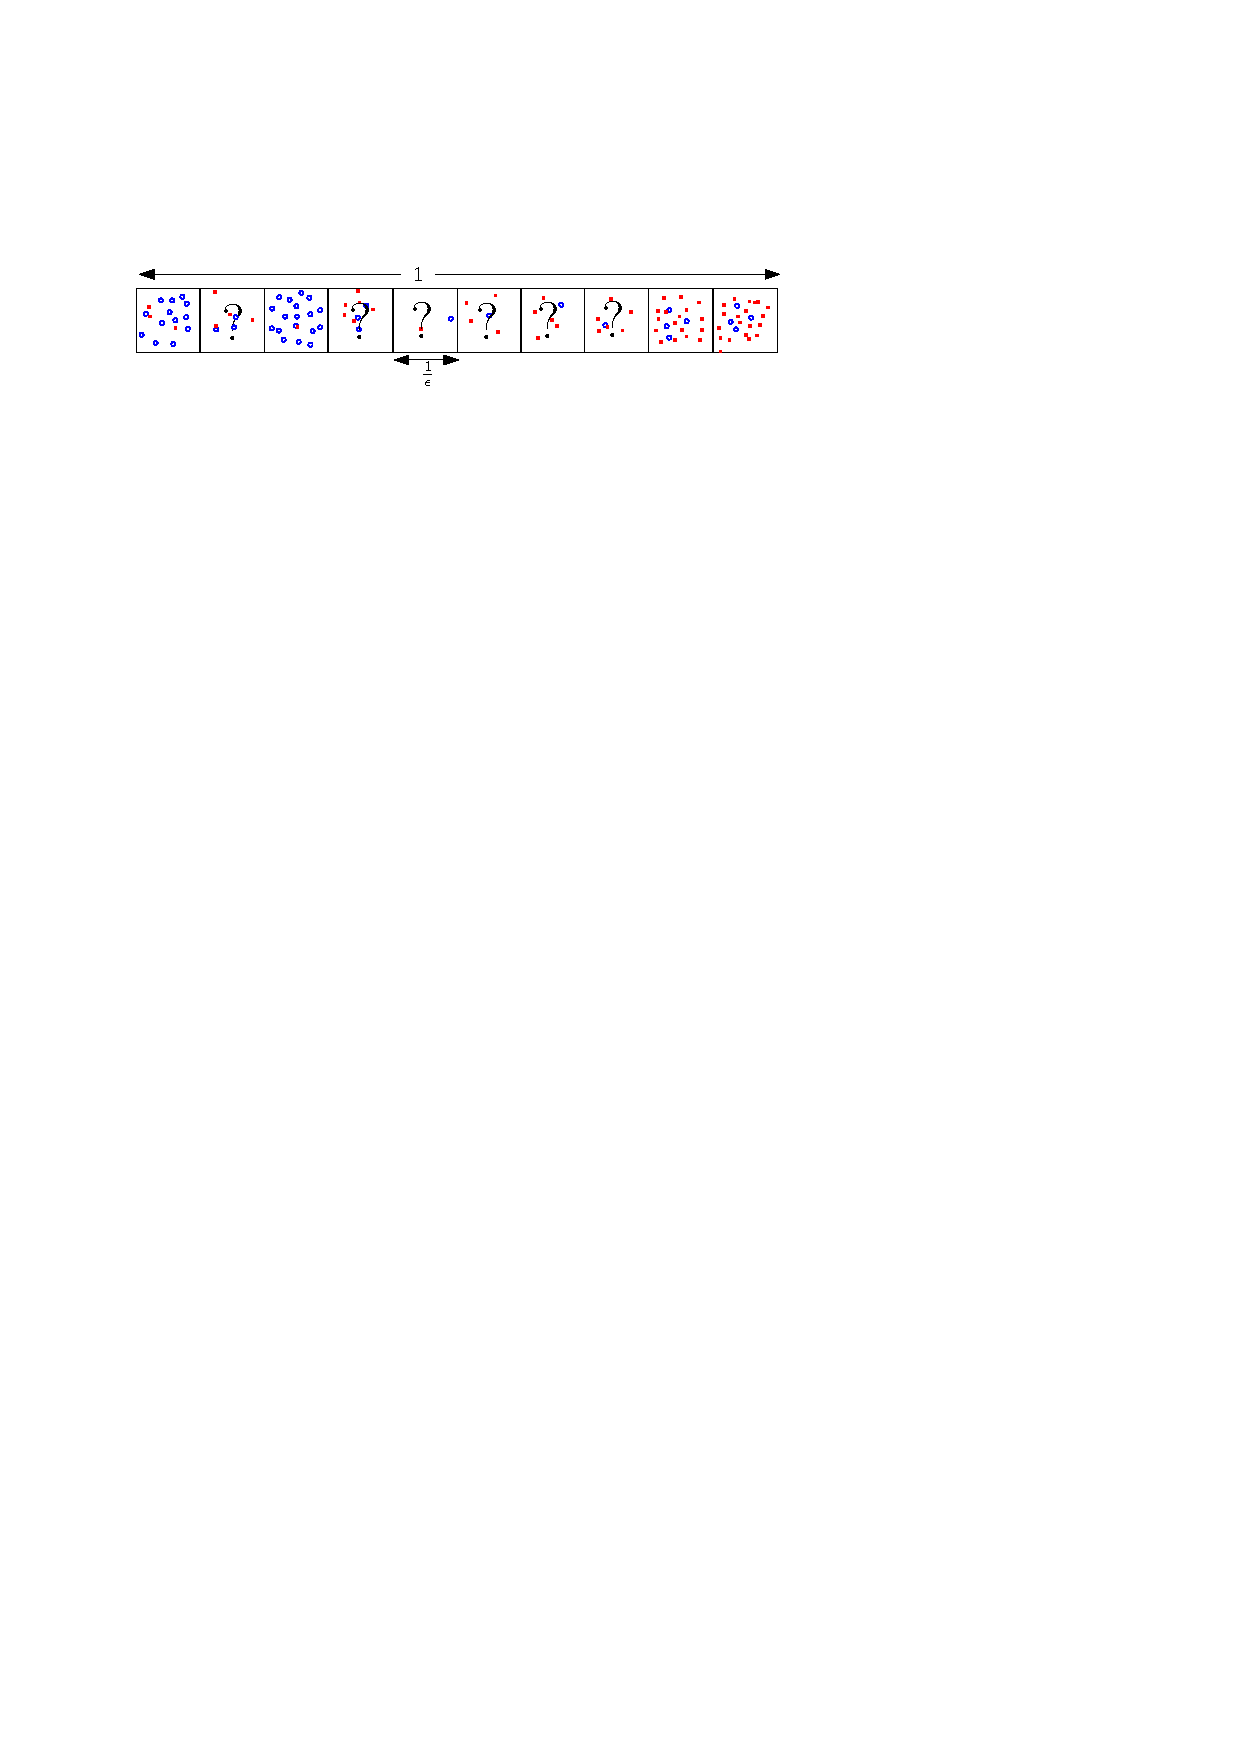
\includegraphics[scale=1.5]{texs/simple_classification.pdf}
   \caption{Visualization of the naive 1D classification}
\label{fig:simple_classification}

\end{figure}






\section{KWIK Inverse Reinforcement Learning Protocol}


We now present the reduction of IRL to KWIK classification. 
\begin{assumption}
We assume that the MDP is specified using the $\vec{\Phi}_Q$ parametrization as discussed in Section ~\ref{sec:formal_generalization}. 
\end{assumption}

While often it is the case that the problem is parametrized in terms of $\vec{\Phi}_R$, that is the rewards, here we follow the approach of \citet{DBLP:conf/icra/SilverBS12} in \textit{directly} assigning long-term cost parametrization to the decisions taken. Note that this by default encodes the MDP structure. We might however be interested in beginning with the $\vec{\Phi}_R$ parametrization which we will leave for future work. \\

\begin{assumption}
$\forall (s,a) \in \mathcal{S} \times \mathcal{A}$,  $||\vec{\Phi}_Q(s,a)||_2 \leq 1$  
\end{assumption}

The above assumption is valid because any parametrization that we begin with can be made to satisfy this by a simple scaling \textit{without  changing the task at hand}.\\


At any state $s \in \mathcal{S}$, the learner is presented with a set of at most $|\mathcal{A}|$ actions of which the learner is required to pick an $\epsilon-$optimal action. Let $\vec{\theta}_E$ be the unknown weight vector for the rewards.  We assume that the learner has access to a KWIK classification algorithm $\mathcal{C}$ whose input space is $\mathbb{R}^k$. For some $a^*,a' \in \mathcal{A}$, we expect the classifier to predict $\text{SGN}[\vec{\theta}_E \cdot(\vec{\Phi}_Q(s,a^*) - \vec{\Phi}_Q(s,a'))]$ given $(\vec{\Phi}_Q(s,a^*) - \vec{\Phi}_Q(s,a'))$ as input. 

\begin{assumption}
We will assume that the input to the classifier is always scaled to a magnitude of 1. 
\end{assumption}

The above assumption does not change our problem because scaling $\vec{\Phi}_Q(s,a^*) - \vec{\Phi}_Q(s,a')$ to \[\frac{\vec{\Phi}_Q(s,a^*) - \vec{\Phi}_Q(s,a')}{||\vec{\Phi}_Q(s,a^*) - \vec{\Phi}_Q(s,a') ||_2}\]
does not change the sign of $\text{SGN}[\vec{\theta}_E \cdot(\vec{\Phi}_Q(s,a^*) - \vec{\Phi}_Q(s,a'))]$.
That is,

\[
\text{SGN} \left[ \frac{\vec{\Phi}_Q(s,a^*) - \vec{\Phi}_Q(s,a')}{||\vec{\Phi}_Q(s,a^*) - \vec{\Phi}_Q(s,a') ||_2}\right]
=\text{SGN} \left[\vec{\Phi}_Q(s,a^*) - \vec{\Phi}_Q(s,a') \right] 
\]

 Thus, in the rest of the discussion we assume that the input to the classifier is scaled appropriately without explicitly mentioning it. \\
 
\begin{lemma}
\label{lemma:diam}
$\forall (s,a^*), (s,a') \in \mathcal{S} \times \mathcal{A}$
\begin{equation}
||\vec{\Phi}_Q(s,a^*) - \vec{\Phi}_Q(s,a') ||_2 \leq 2
\end{equation}
\end{lemma} 
 
 

\begin{thm}
\label{thm:kwik_converse}
If the accuracy parameter of $\mathcal{C}$ is set at
\[
\frac{\epsilon}{2(|\mathcal{A}|-1)}
\]
then:

 for the input $\vec{\Phi}_Q(s,a^*) - \vec{\Phi}_Q(s,a')$, if
\begin{equation}
\vec{\theta}_E \cdot (\vec{\Phi}_Q(s,a^*) - \vec{\Phi}_Q(s,a')) \geq  \frac{\epsilon}{|\mathcal{A}|-1}
\end{equation}

then $\mathcal{C}$ predicts $+1$ if it makes a valid prediction;

and if
\begin{equation}
\vec{\theta}_E \cdot (\vec{\Phi}_Q(s,a') - \vec{\Phi}_Q(s,a^*)) \geq  \frac{\epsilon}{|\mathcal{A}|-1}
\end{equation}
then $\mathcal{C}$ predicts $-1$ if it makes a valid prediction.

\end{thm} 
 
 
\begin{proof}
If 
\begin{equation}
\vec{\theta}_E \cdot (\vec{\Phi}_Q(s,a^*) - \vec{\Phi}_Q(s,a')) \geq  \frac{\epsilon}{|\mathcal{A}|-1}
\end{equation}
then
\[
\begin{array}{rcl}
{\vec{\theta}_E \cdot \displaystyle \frac{(\vec{\Phi}_Q(s,a^*) - \vec{\Phi}_Q(s,a'))}{||\vec{\Phi}_Q(s,a^*) - \vec{\Phi}_Q(s,a')||_2 } } & 
>& \displaystyle \frac{\epsilon}{|\mathcal{A}-1|} \times \frac{1}{||\vec{\Phi}_Q(s,a^*) - \vec{\Phi}_Q(s,a')||_2} \\
&&\\
&\geq& \displaystyle\frac{\epsilon}{|\mathcal{A}-1|}  \times \frac{1}{2}
\end{array}
\]
The first inequality here comes from the assumption we made. The second inequality comes from Lemma ~\ref{lemma:diam}. Thus, the dot product between the normalized input and the true weight vector is strictly greater than $\frac{\epsilon}{2(|\mathcal{A}-1|)}$ which is the accuracy parameter of the classifier. Hence, we know that the KWIK classification algorithm, if at all made a valid prediction, had to make the right prediction, which is $+1$.

We skip the proof for the second result as it is identical.
\end{proof} 
 
 
\begin{thm}
\label{thm:kwik_condition}
If the accuracy parameter of $\mathcal{C}$ is set at
\[
\frac{\epsilon}{2(|\mathcal{A}|-1)}
\]
then:

 for the input $\vec{\Phi}_Q(s,a^*) - \vec{\Phi}_Q(s,a')$, if $\mathcal{C}$ predicts $+1$, then 
\begin{equation}
\vec{\theta}_E \cdot (\vec{\Phi}_Q(s,a^*) - \vec{\Phi}_Q(s,a')) \geq - \frac{\epsilon}{|\mathcal{A}|-1}
\end{equation}

If $\mathcal{C}$ predicts $-1$, then
\begin{equation}
\vec{\theta}_E \cdot (\vec{\Phi}_Q(s,a') - \vec{\Phi}_Q(s,a^*)) \geq - \frac{\epsilon}{|\mathcal{A}|-1}
\end{equation}

\end{thm}

\begin{proof}
The proof for the above results are identical. Hence, we prove the first result. Let the prediction made by the KWIK classifier be $+1$. Assume on the contrary that 
\[
\vec{\theta}_E \cdot (\vec{\Phi}_Q(s,a^*) - \vec{\Phi}_Q(s,a')) < - \frac{\epsilon}{|\mathcal{A}|-1}
\]
Then, from Theorem ~\ref{thm:kwik_converse}, we know that the classifier has to have output $-1$.  Since this contradicts the fact that $\mathcal{C}$ predicted $+1$, we prove that our assumption is wrong. 
\end{proof}

Thus, whenever the classifier makes a valid prediction and favors one action over the other, we see that the preferred action cannot be worse than the  other action by a value of more than $\epsilon/(|\mathcal{A}|-1)$. 


If the classifier is unable to predict, and instead outputs a $\perp$ we request expert advice in the form of a preference over these pair of actions. We note that we could study various other modifications of this algorithm, where the expert only provides knowledge about the best action amongst all actions instead of pairwise preferences. 


We present below the protocol followed by the learner in order to choose the $\epsilon-$optimal action 
if it takes a decision autonomously. 


\begin{algorithm}[H]
\caption{KWIK Inverse Reinforcement Learning Protocol}
\label{alg:imilearn}
\begin{algorithmic}
\Require {Teacher $\mathcal{T}(\epsilon_Y)$ with true weight vector for rewards ${\vec{\theta}}_E$, Admissible KWIK Classifier $\mathcal{C}(\frac{\epsilon}{2(|\mathcal{A}|-1)},\delta)$ with weight estimate for rewards $\hat{\vec{\theta}}$}
    \For{$t=1,2,\hdots$}
        \State $s = $ Current State of the Environment
        \State $\hat{a}_{best} = a_1$
        \For{i = $2, \hdots |\mathcal{A}|$}
            \State Present $\vec{\Phi}_Q(s,a_i) - \vec{\Phi}_Q(s,\hat{a}_{best})$ to $\mathcal{C}$
            \If{Output of $\mathcal{C} = \perp$}
                \State Present  $\vec{\Phi}_Q(s,a_i) - \vec{\Phi}_Q(s,\hat{a}_{best})$ to  $\mathcal{T}$
               \State $\mathcal{T}$ outputs  $\text{SGN}[{\vec{\theta}}_E \cdot(\vec{\Phi}_Q(s,a_i) - \vec{\Phi}_Q(s,\hat{a}_{best}))]$

                \State $\mathcal{C}$ learns from output of $\mathcal{T}$ and updates $\hat{\vec{\theta}}$
                \If{Output of $\mathcal{T} = +1$}
                    \State $\hat{a}_{best} = a_i$
                \EndIf
            
            \Else
                \State $\mathcal{C}$ outputs $\text{SGN}[\hat{\vec{\theta}}_E \cdot(\vec{\Phi}_Q(s,a_i) - \vec{\Phi}_Q(s,\hat{a}_{best}))]$
                \If{Output of $\mathcal{C} = +1$}
                    \State $\hat{a}_{best} = a_i$
                \EndIf
            \EndIf
        \EndFor
        \State Perform $\hat{a}_{best}$
    \EndFor
\end{algorithmic}
\end{algorithm}



In Algorithm ~\ref{alg:imilearn}, at any state the learner scans all the possible actions (which is at most $|\mathcal{A}|$) and maintains a candidate action that it considers to be the best amongst the actions that have been iterated through. The correctness of this algorithm would follow if we show that after iterating over all the actions, if the algorithm has not queried the teacher, it always chooses an $\epsilon$-optimal action. We prove the following lemma from which the above statement follows directly by setting $i=|\mathcal{A}|$. 

\begin{thm} After iterating over the first $i$ actions, if the algorithm has not made any queries, the candidate action picked by the algorithm is $(i-1)\displaystyle\frac{\epsilon}{|\mathcal{A}|-1}-$ optimal with respect to the best action amongst the first $i$ actions.
\end{thm}

\begin{proof}
The claim trivially holds good when $i=1$. 
For any arbitrary round $i < |\mathcal{A}|$ assume that the claim is true. This is our inductions hypothesis. That is, if $\hat{a}_i$ is the candidate action picked by the algorithm, and $a_i^*$ is the best action amongst the first $i$ actions, then:
\begin{equation}\label{eq:ind}
\vec{\theta}_E\cdot \vec{\Phi}_Q(s,\hat{a}_i) \geq \vec{\theta}_E\cdot \vec{\Phi}_Q(s,a_i^*) - (i-1)\frac{\epsilon}{|\mathcal{A}|-1} 
\end{equation}

If the algorithm chose $a_{i+1}$ over $\hat{a}_i$, we know from Theorem ~\ref{thm:kwik_condition}  that
\begin{equation}\label{eq:changeaction}
\vec{\theta}_E\cdot \vec{\Phi}_Q(s,a_{i+1}) \geq \vec{\theta}_E\cdot \vec{\Phi}_Q(s,\hat{a}_i) - \frac{\epsilon}{|\mathcal{A}|-1}
\end{equation}


If the decision of choosing $a_{i+1}$ over $\hat{a}_i$ were to be inconsistent with our claim, $a_{i+1}$ must not be an $i \frac{\epsilon}{|\mathcal{A}|-1}$-optimal action (among the first $i+1$ actions). Then $a^*$ must \textit{still} be the best action amongst the first $i+1$ actions. However, from inequalities (~\ref{eq:ind}) and (~\ref{eq:changeaction}), we can see that:
\[
\vec{\theta}_E\cdot \vec{\Phi}_Q(s,{a}_{i+1}) \geq \vec{\theta}_E\cdot \vec{\Phi}_Q(s,a^*) - i\frac{\epsilon}{|\mathcal{A}|-1}
\]
which makes $a_{i+1}$ an $i \frac{\epsilon}{|\mathcal{A}|-1}$-optimal action amongst the first $i+1$ actions, which is a contradiction. Thus, if the algorithm chose  $a_{i+1}$ over $\hat{a}_i$, it must have been right.

On the other hand, if the algorithm still chose $\hat{a}_i$ over $a_{i+1}$, it would be inconsistent with our claim only if $a_{i+1}$ was the best action amongst the $i+1$ actions and if $\hat{a}_i$ was not sufficiently optimal. That is,

\begin{equation}\label{eq:notoptimal}
\vec{\theta}_E\cdot \vec{\Phi}_Q(s,\hat{a}_{i}) < \vec{\theta}_E\cdot \vec{\Phi}_Q(s,a_{i+1}) - i\frac{\epsilon}{|\mathcal{A}|-1}
\end{equation}

However, this implies a much weaker inequality:
\[
\vec{\theta}_E\cdot \vec{\Phi}_Q(s,\hat{a}_{i}) < \vec{\theta}_E\cdot \vec{\Phi}_Q(s,a_{i+1}) - \frac{\epsilon}{|\mathcal{A}|-1}
\]
which would have ensured that the KWIK classifier indicated that $a_{i+1}$
was a better action (Lemma ~\ref{thm:kwik_converse}). Hence, by induction we show that the lemma holds good for all $i = 1, \hdots |\mathcal{A}|$. 

\end{proof}

\begin{corr}
After scanning over all the actions, if the algorithm has not made any queries, the candidate action picked by the algorithm is an ${\epsilon}-$ optimal action.
\end{corr}


\section{Multidimensional KWIK Classifier}
We discuss in this section preliminary ideas on how a classifier could be designed for a $k-$dimensional input space. \\


Let us describe a naive idea first. We follow an idea similar to that of the 1-D classifier discussed in Section ~\ref{sec:simple}. The idea is to split the input space into $N$ appropriate subspaces, and make predictions in these subspaces only after making sufficient number of queries in each of them.
We want each segment to fail with atmost $\delta/N$ probability so that the total failure probability is atmost $\delta$ (Lemma ~\ref{lemma:union_bound}). From Lemma $~\ref{lemma:coinlearn}$, each subspace will thus require $\frac{1}{\epsilon_Y^2} \ln \left( \frac{N}{\delta}\right)$ points to ensure that the majority of labels is correct. Thus, we will make as many queries as:
\begin{equation}
\label{eq:kwiksegment}
N \times\frac{1}{\epsilon_Y^2} \ln \left( \frac{N}{\delta}\right)
\end{equation}

The constraint with splitting the space is that the subspaces must be of width not more than $\epsilon$. We could come up with many different ways of splitting the unit hypersphere surface. We skip discussing these ideas here as they do not form the core of our discussion. However, we must note that such a splitting will always be of of the order $\mathcal{O}(1/\epsilon^k)$. Thus, we will end up making queries of the order:

\begin{equation}
\label{eq:kwiksegment}
\frac{1}{\epsilon^k\epsilon_Y^2} \ln \left( \frac{1}{\epsilon^k\delta}\right)
\end{equation}

which is \textit{\textbf{exponential}}!

Our aim in this discussion is to gain insights about how we can \textit{characterize} regions in the input space by generalizing from experience across the space and not just from the local neighborhood. This might \textit{perhaps} lead us to a polynomial bound. 



\begin{figure}[H]
\centering
   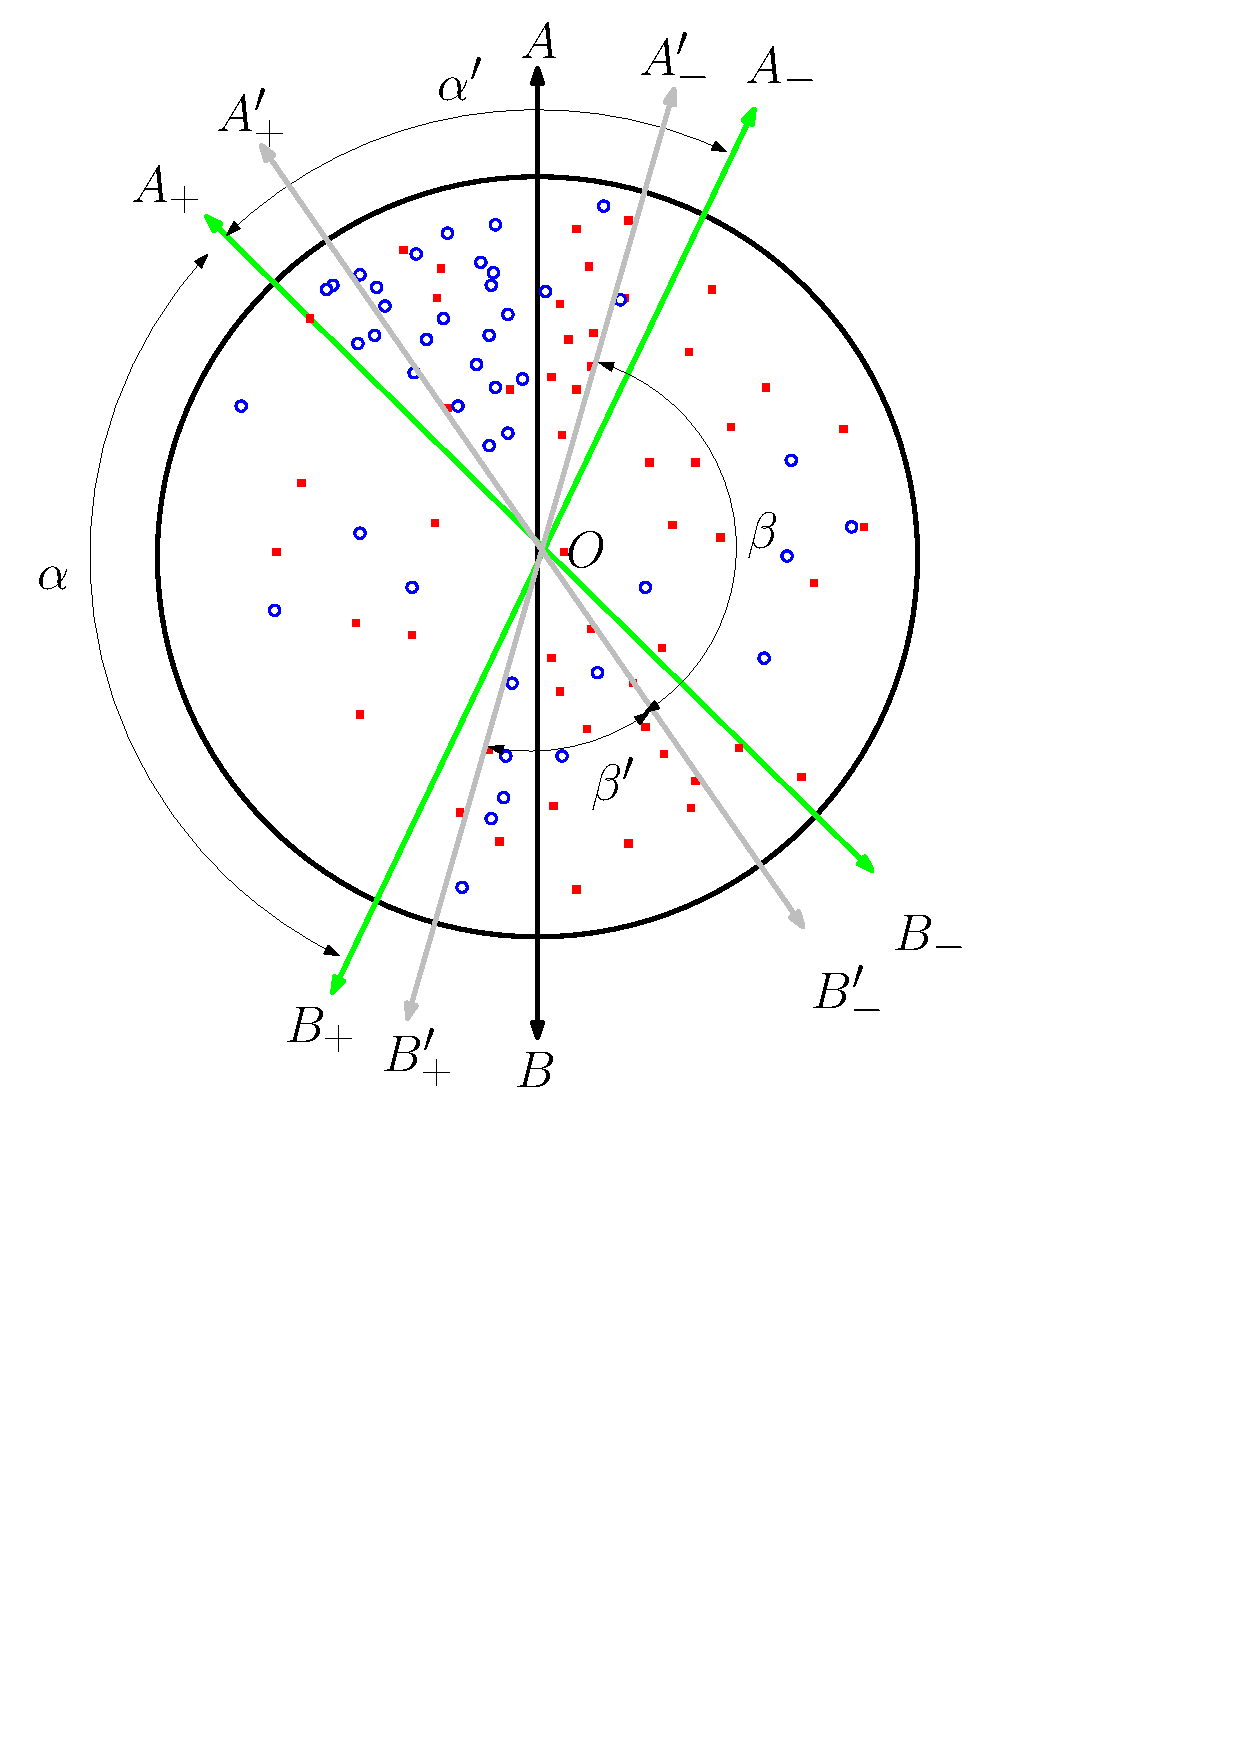
\includegraphics[scale=0.6]{texs/classification.pdf}
   \caption{Visualization of the k-D classification}
\label{fig:classification}
\end{figure}


\begin{remark}
The KWIK classifier imposes stricter restrictions on the learner in imitation learning than that is required of the learner for it to be near-optimal. 
\end{remark}
Consider the space of input points which are not normalized. Visually, the subspace where infinitely many mistakes are allowed by the near-optimal learner is a cylindrical margin around the separating hyperplane. The cylinder is of radius $\epsilon/2(|\mathcal{A}-1|)$. However, the classifier $\mathcal{C}$ allows infinitely many mistakes only in a conical region centred at the origin with the base subtended at the unit hypersphere of radius $\epsilon/2(|\mathcal{A}-1|)$. There is space outside of this cone that can still be misclassified for the near-optimality requirements of the learner. This discrepancy comes from the fact that the classifier takes in normalized inputs.
However the discrepancy is not invalid in any sense because,  the classifier is known to pass through the origin, and any sort of perturbation will be only with respect to its `angle'; if the classifier is perturbed the space it sweeps is only a conical region and hence we must allow errors to occur only in this region. \\